\documentclass[12pt]{article}
\usepackage[english]{babel}
\usepackage[utf8]{inputenc}
\usepackage{amsmath, amssymb, amsthm}
\usepackage{graphicx}
\usepackage{hyperref}
\usepackage{geometry}
\usepackage{xcolor}
\usepackage{tikz}

\setlength{\topmargin}{0pt}
\setlength{\headsep}{0pt}
\textheight = 600pt

\title{Graph Theory \\ Homework 4}
\author{Ben Kallus and Maddy LaPoint}
\date{Due Friday, February 19}

\begin{document}
\pagecolor{black}
\color{white}
\maketitle

\noindent{\bf 2.2}

{\bf (a)}

\medskip
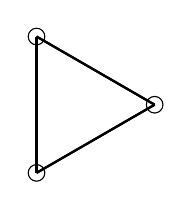
\begin{tikzpicture}
\draw[fill=white] (1.0, 0.0) circle (3pt);
\draw[fill=white] (-0.5, 0.866) circle (3pt);
\draw[fill=white] (-0.5, -0.866) circle (3pt);

\draw[thick] (1.0, 0.0) -- (-0.5, -0.866);
\draw[thick] (1.0, 0.0) -- (-0.5, 0.866);
\draw[thick] (-0.5, 0.866) -- (1.0, 0.0);
\draw[thick] (-0.5, 0.866) -- (-0.5, -0.866);
\draw[thick] (-0.5, -0.866) -- (1.0, 0.0);
\draw[thick] (-0.5, -0.866) -- (-0.5, 0.866);
\end{tikzpicture}



\bigskip
{\bf (b)}

\medskip
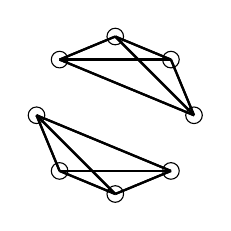
\begin{tikzpicture}
\draw[fill=white] (1.0, 0.0) circle (3pt);
\draw[fill=white] (0.707, 0.707) circle (3pt);
\draw[fill=white] (0.0, 1.0) circle (3pt);
\draw[fill=white] (-0.707, 0.707) circle (3pt);
\draw[fill=white] (-1.0, 0.0) circle (3pt);
\draw[fill=white] (-0.707, -0.707) circle (3pt);
\draw[fill=white] (-0.0, -1.0) circle (3pt);
\draw[fill=white] (0.707, -0.707) circle (3pt);

\draw[thick] (1.0, 0.0) -- (-0.707, 0.707);
\draw[thick] (1.0, 0.0) -- (0.707, 0.707);
\draw[thick] (1.0, 0.0) -- (0.0, 1.0);
\draw[thick] (0.707, 0.707) -- (1.0, 0.0);
\draw[thick] (0.707, 0.707) -- (-0.707, 0.707);
\draw[thick] (0.707, 0.707) -- (0.0, 1.0);
\draw[thick] (0.0, 1.0) -- (1.0, 0.0);
\draw[thick] (0.0, 1.0) -- (-0.707, 0.707);
\draw[thick] (0.0, 1.0) -- (0.707, 0.707);
\draw[thick] (-0.707, 0.707) -- (1.0, 0.0);
\draw[thick] (-0.707, 0.707) -- (0.707, 0.707);
\draw[thick] (-0.707, 0.707) -- (0.0, 1.0);
\draw[thick] (-1.0, 0.0) -- (-0.0, -1.0);
\draw[thick] (-1.0, 0.0) -- (0.707, -0.707);
\draw[thick] (-1.0, 0.0) -- (-0.707, -0.707);
\draw[thick] (-0.707, -0.707) -- (0.707, -0.707);
\draw[thick] (-0.707, -0.707) -- (-1.0, 0.0);
\draw[thick] (-0.707, -0.707) -- (-0.0, -1.0);
\draw[thick] (-0.0, -1.0) -- (0.707, -0.707);
\draw[thick] (-0.0, -1.0) -- (-1.0, 0.0);
\draw[thick] (-0.0, -1.0) -- (-0.707, -0.707);
\draw[thick] (0.707, -0.707) -- (-0.0, -1.0);
\draw[thick] (0.707, -0.707) -- (-1.0, 0.0);
\draw[thick] (0.707, -0.707) -- (-0.707, -0.707);
\end{tikzpicture}

\bigskip
{\bf (c)}

\medskip
\begin{tikzpicture}
\draw[fill=white] (1.0, 0.0) circle (3pt);
\draw[fill=white] (0.309, 0.951) circle (3pt);
\draw[fill=white] (-0.809, 0.588) circle (3pt);
\draw[fill=white] (-0.809, -0.588) circle (3pt);
\draw[fill=white] (0.309, -0.951) circle (3pt);
\end{tikzpicture}


\bigskip
{\bf (d)}

\medskip
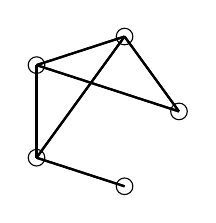
\begin{tikzpicture}
\draw[fill=white] (1.0, 0.0) circle (3pt);
\draw[fill=white] (0.309, 0.951) circle (3pt);
\draw[fill=white] (-0.809, 0.588) circle (3pt);
\draw[fill=white] (-0.809, -0.588) circle (3pt);
\draw[fill=white] (0.309, -0.951) circle (3pt);

\draw[thick] (1.0, 0.0) -- (0.309, 0.951);
\draw[thick] (1.0, 0.0) -- (-0.809, 0.588);
\draw[thick] (0.309, 0.951) -- (-0.809, -0.588);
\draw[thick] (0.309, 0.951) -- (-0.809, 0.588);
\draw[thick] (0.309, 0.951) -- (1.0, 0.0);
\draw[thick] (-0.809, 0.588) -- (0.309, 0.951);
\draw[thick] (-0.809, 0.588) -- (-0.809, -0.588);
\draw[thick] (-0.809, 0.588) -- (1.0, 0.0);
\draw[thick] (-0.809, -0.588) -- (0.309, 0.951);
\draw[thick] (-0.809, -0.588) -- (0.309, -0.951);
\draw[thick] (-0.809, -0.588) -- (-0.809, 0.588);
\draw[thick] (0.309, -0.951) -- (-0.809, -0.588);
\end{tikzpicture}

\bigskip
\noindent{\bf 2.3}

    $K_7 \cup K_5$ has order 12, size 31, and each of its vertices is either degree 4 or degree 6. Thus, such a graph would have 5 vertices of degree 4.

\bigskip
\noindent{\bf 2.6}

{\bf Proposition:} If a graph of order $3n$ ($n \geq 1$) has $n$ vertices of each of the degrees $n-1$, $n$, and $n+1$, then $n$ is even.
\begin{proof}
    Let $n \in \mathbb N$, and let $G$ be a graph of order $3n$ with $n$ vertices of each of the degrees $n-1$, $n$, and $n+1$.
    Suppose, toward a contradiction, that the order of $G$ is odd.
    Then, $G$ contains $2n$ even vertices, and $n$ odd vertices.
    Since $n$ is odd, this violates the Handshaking Lemma.
    Thus, if a graph of order $3n$ ($n \geq 1$) has $n$ vertices of each of the degrees $n-1$, $n$, and $n+1$, then $n$ is even.
\end{proof}

\bigskip
\noindent{\bf 2.12}

{\bf Proposition:} If $G$ is a graph of order $n$ such that $\Delta(G) + \delta(G) \geq n - 1$, then $G$ is connected and $\text{diam}(G) \leq 4$.
\begin{proof}
    Let $G$ be a graph of order $n$ such that $\Delta(G) + \delta(G) \geq n - 1$.
    Let $x$ and $y$ be distinct vertices in $G$, and let $u$ be a vertex of maximum degree in $G$.
    Consider the case in which $xy \in E(G)$.
    Then, $x$ and $y$ are connected by a path of length 1, so $d_G(u,v) = 1$.
    Now, consider the case in which $xy \notin E(G)$.
    Since $\Delta(G) + \delta(G) \geq n - 1$, $\deg(u) + \deg(x) \geq n - 1$.
    Thus, there exists a vertex $w$ adjacent to both $u$ and $x$.
    By a symmetric argument, there exists a vertex $t$ adjacent to both $u$ and $y$.
    Thus, $(x, w, u, t, y)$ is a walk of length 4 in $G$ that connects $x$ and $y$.
    Thus, $G$ is connected, and the diamater of $G$ is 4.
\end{proof}


{\bf Proposition:} The bound given in the previous proof is sharp.
\begin{proof}
    Consider the disconnected graph $G = K_2 \cup K_1$.
    Since $1 + 0 \geq 3 - 2$, $$\Delta(G) + \delta(G) \geq n - 1.$$
    Thus, the bound given in the previous proof is sharp.
\end{proof}

\newpage
\noindent{\bf 2.18}

Observe that $v_8$ must have degree 4:

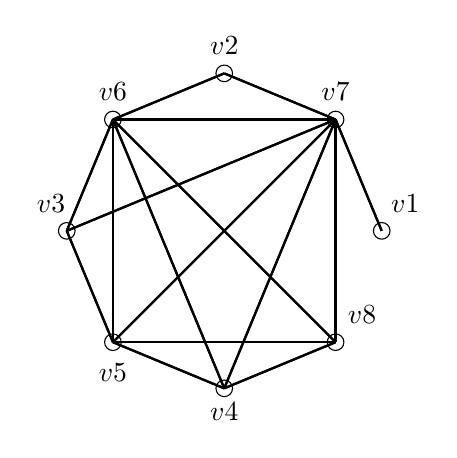
\begin{tikzpicture}
\draw[fill=white] (2.0, 0.0) circle (3pt);
\node at (2.3, 0.35) {$v1$};
\draw[fill=white] (1.414, 1.414) circle (3pt);
\node at (1.414, 1.7639999999999998) {$v7$};
\draw[fill=white] (0.0, 2.0) circle (3pt);
\node at (0.0, 2.35) {$v2$};
\draw[fill=white] (-1.414, 1.414) circle (3pt);
\node at (-1.414, 1.7639999999999998) {$v6$};
\draw[fill=white] (-2.0, 0.0) circle (3pt);
\node at (-2.2, 0.35) {$v3$};
\draw[fill=white] (-1.414, -1.414) circle (3pt);
\node at (-1.414, -1.8) {$v5$};
\draw[fill=white] (-0.0, -2.0) circle (3pt);
\node at (0.0, -2.3) {$v4$};
\draw[fill=white] (1.414, -1.414) circle (3pt);
\node at (1.75, -1.064) {$v8$};

\draw[thick] (2.0, 0.0) -- (1.414, 1.414);
\draw[thick] (1.414, 1.414) -- (-1.414, -1.414);
\draw[thick] (1.414, 1.414) -- (-1.414, 1.414);
\draw[thick] (1.414, 1.414) -- (-2.0, 0.0);
\draw[thick] (1.414, 1.414) -- (0.0, 2.0);
\draw[thick] (1.414, 1.414) -- (-0.0, -2.0);
\draw[thick] (1.414, 1.414) -- (2.0, 0.0);
\draw[thick] (0.0, 2.0) -- (1.414, 1.414);
\draw[thick] (0.0, 2.0) -- (-1.414, 1.414);
\draw[thick] (-1.414, 1.414) -- (-1.414, -1.414);
\draw[thick] (-1.414, 1.414) -- (-2.0, 0.0);
\draw[thick] (-1.414, 1.414) -- (0.0, 2.0);
\draw[thick] (-1.414, 1.414) -- (-0.0, -2.0);
\draw[thick] (-1.414, 1.414) -- (1.414, -1.414);
\draw[thick] (-1.414, 1.414) -- (1.414, 1.414);
\draw[thick] (-2.0, 0.0) -- (1.414, 1.414);
\draw[thick] (-2.0, 0.0) -- (-1.414, -1.414);
\draw[thick] (-2.0, 0.0) -- (-1.414, 1.414);
\draw[thick] (-1.414, -1.414) -- (-1.414, 1.414);
\draw[thick] (-1.414, -1.414) -- (-2.0, 0.0);
\draw[thick] (-1.414, -1.414) -- (-0.0, -2.0);
\draw[thick] (-1.414, -1.414) -- (1.414, -1.414);
\draw[thick] (-1.414, -1.414) -- (1.414, 1.414);
\draw[thick] (-0.0, -2.0) -- (-1.414, -1.414);
\draw[thick] (-0.0, -2.0) -- (-1.414, 1.414);
\draw[thick] (-0.0, -2.0) -- (1.414, 1.414);
\draw[thick] (-0.0, -2.0) -- (1.414, -1.414);
\draw[thick] (1.414, -1.414) -- (-0.0, -2.0);
\draw[thick] (1.414, -1.414) -- (-1.414, -1.414);
\draw[thick] (1.414, -1.414) -- (-1.414, 1.414);
\draw[thick] (1.414, 1.414) -- (1.414, -1.414);
\end{tikzpicture}

\bigskip
\noindent{\bf 2.19}



\end{document}